\chapter{Conclusion}\label{chap:conclusion}

\section{Evaluation of Results}
To summarize the research conducted up to this point, a GPU-supported parallel Andersen based pointer analysis, PTAGPU, was implemented on top of LLVM and the SVF framework using the NVIDIA CUDA SDK.
PTAGPU was both tested for correctness and performance in comparison to established CPU-based pointer analyses in multiple benchmarks and hardware combinations.
The primary research question was to what extent such an implementation presents advantages or disadvantages over other analyses that are not strictly parallel in nature.

The experimental results presented in \autoref{sec:results} indicate that PTAGPU is a viable implementation to improve the performance of a whole program field-sensitive pointer analysis without sacrificing precision of the analysis.
PTAGPU achieved an average speedup of 1.60 across 15 benchmarks over the SVF wavediff algorithm. Since the individual benchmarks with lower speedups are almost entirely smaller programs, the absolute time saved by using PTAGPU was 28 minutes and 59 seconds over the total 1 hour 07 minutes and 30 seconds required by wavediff to analyze all 16 programs. In terms of absolute time, the speedup factor was 1.75.
This represents a meaningful improvement over the CPU algorithm. 
Unfortunately this does not include the linux benchmark, as the analysis did not fit into graphics memory and did not finish within a reasonable amount of time.
Although enough unified memory was available, the analyis of the linux source code did become impeded by excessive page faults as illustrated in \autoref{sec:results}.
Judging from the wavediff analysis of the linux kernel, roughly 300 GiB of memory are required for a successful whole program field-sensitive pointer analysis, which is currently impossible to compute on a single GPGPU.

One key insight from the experimental results was, that there are no trivial prior indicators for analysis runtime, since program structure are seemingly more influential on analysis runtime than lines of code, nodes in the constraint graph or size of the compiled program.
This is supported by prior research from \cite{mendez2012gpu}, where the selected benchmark programs - some of which overlap with the selected benchmark programs of this thesis - also had vastly different speedups for the GPU-based analysis over the CPU-based analyses. 

Although the results indicate that PTAGPU generally outperforms the CPU counterparts in larger benchmarks, it should be acknowledged that it is difficult to establish a fair comparison betwenn CPU and GPU pointer analysis implementations.
Both in terms of upfront cost and power consumption both implementations are vastly different. While the SVF wavediff algorithm can be executed on almost any modern computer with sufficient main memory, PTAGPU requires specialized hardware. Especially for larger analyses, a GPU with enough graphics memory is required for an efficient analysis with PTAGPU.

Concluding, PTAGPU was capable of meaningfully improving the performance of a whole program field-sensitive pointer analysis.
The main advantages lie with relatively large programs that are built using a flat code structure, where PTAGPU achieves a respectable speedup over CPU-based pointer analyses.
The disadvantages are that using GPUs for a pointer analysis always introduces an overhead for graphics memory management and conversion of input data into a format suitable for the GPU.
This makes using GPUs for analyzing small programs (less than 1MB in size) inefficient.
For optimal performance PTAGPU also requires that the entire analysis fits into graphics memory, which prevents some of the largest software projects, such as the linux kernel, from being analyzed by PTAGPU.

\section{Future Work}
\subsection{Partitioning Workloads}
\subsection{Hybrid Cycle Detection}
\section{Discussion}

\appendix

\chapter{Raw Data}

\begin{table}[ht]
    \tiny
    \begin{tabular}{rrrrrrrrr}
        \toprule
           & file         & GPU memory MiB & filesize MB & wavediff-t   & naiveander-t & \# nodes & \# edges & version \\
        \midrule
        1  & bash         & 1024           & 5.400       & 16222.113    & 102195.752   & 238      & 77       & 6.4     \\
        2  & bison        & 260            & 3.400       & 18977.376    & 119999.054   & 146      & 59       & 3.8     \\
        3  & diff         & 71             & 1.300       & 1469.056     & 1561.577     & 54       & 17       & 2.4.54  \\
        4  & git          & 21467          & 25.000      & 557953.924   & 33404492.853 & 869      & 379      & 3.2.1   \\
        5  & htop         & 93             & 1.600       & 2912.693     & 5696.107     & 48       & 20       & 1.5.2   \\
        6  & httpd        & 160            & 1.400       & 5321.631     & 2889.208     & 169      & 95       & 3.8     \\
        7  & nano         & 7              & 0.298       & 87.438       & 98.500       & 6        & 2        & 7.0.5   \\
        8  & perl         & 3999           & 4.900       & 103338.824   & 2688610.846  & 445      & 206      & 5.37.3  \\
        9  & php          & 27561          & 52.000      & 645697.175   & 6530636.248  & 1582     & 611      & 5.14    \\
        10 & postgres     & 16430          & 18.000      & 997355.718   & 6481597.401  & 1432     & 721      & 5.1.16  \\
        11 & python       & 9016           & 21.000      & 536515.479   & 1731373.999  & 742      & 313      & 9.0     \\
        12 & redis-server & 207            & 4.800       & 8679.144     & 4834.759     & 207      & 67       & 14.4    \\
        13 & vim          & 11966          & 7.700       & 1052995.525  & NaN          & 696      & 280      & 3.10.6  \\
        14 & vmlinux      & NaN            & 72.000      & 32100566.652 & NaN          & 4464     & 2206     & 2.37.4  \\
        15 & vmlinux-tiny & 2175           & 5.400       & 91479.697    & 1410004.628  & 393      & 157      & 7.4.31  \\
        16 & zstd         & 454            & 2.300       & 11063.214    & 7958.999     & 280      & 101      & 5.14    \\
        \bottomrule
    \end{tabular}

    \caption[Raw Data of Baseline results for wavediff and naiveander Pointer Analyses]{Raw Data of Baseline results for wavediff and naiveander Pointer Analyses\\Node and Edge count in thousands.}
\end{table}

\begin{table}[ht]
    \tiny
    \begin{tabular}{rrrrrrrrrr}
        \toprule
           & ptagpu-t    & svf init & cuda init & update-k   & main-k       & thrust sort & store-k      & async CPU  & S    \\
        \midrule
        1  & 15489.00    & 366.515  & 2489.389  & 1129.063   & 1324.698     & 743.670     & 858.932      & 5190.693   & 1.05 \\
        2  & 9837.06     & 214.357  & 1650.840  & 830.177    & 234.046      & 675.748     & 54.633       & 4317.114   & 1.93 \\
        3  & 4231.58     & 66.945   & 2065.479  & 103.057    & 33.120       & 379.843     & 23.591       & 953.283    & 0.35 \\
        4  & 4690010.00  & 2190.250 & 17095.315 & 70148.000  & 3968158.215  & 11743.372   & 68373.295    & 538454.710 & 0.12 \\
        5  & 5275.51     & 68.425   & 2053.573  & 229.714    & 202.955      & 433.321     & 41.092       & 1587.968   & 0.55 \\
        6  & 6414.69     & 309.354  & 1481.509  & 303.996    & 42.605       & 511.057     & 8.219        & 1637.408   & 0.83 \\
        7  & 1751.01     & 7.732    & 1533.113  & 1.829      & 3.040        & 45.140      & 1.057        & 94.275     & 0.05 \\
        8  & 45093.40    & 775.915  & 2939.635  & 3457.350   & 6125.819     & 767.334     & 2751.206     & 21457.059  & 2.29 \\
        9  & 64965400.00 & 2809.670 & 20928.407 & 193679.543 & 53783100.092 & 12298.489   & 10732741.786 & 187398.213 & 0.01 \\
        10 & 465527.00   & 2911.590 & 8824.470  & 65379.251  & 192989.575   & 1374.555    & 32019.477    & 135372.093 & 2.14 \\
        11 & 203649.00   & 1344.910 & 4088.639  & 14380.164  & 63762.440    & 16295.704   & 12199.745    & 79598.063  & 2.63 \\
        12 & 11592.50    & 357.262  & 2785.032  & 688.684    & 95.318       & 1158.755    & 42.613       & 3688.319   & 0.75 \\
        13 & 268628.00   & 1166.830 & 9292.169  & 10709.775  & 113872.762   & 947.744     & 20876.445    & 100689.414 & 3.92 \\
        14 & NaN         & NaN      & NaN       & NaN        & NaN          & NaN         & NaN          & NaN        & NaN  \\
        15 & 188315.00   & 654.966  & 2405.784  & 10600.173  & 25890.805    & 12319.814   & 7893.207     & 121492.773 & 0.49 \\
        16 & 13172.60    & 388.764  & 2791.627  & 680.571    & 90.320       & 687.799     & 80.554       & 4526.521   & 0.84 \\
        \bottomrule
    \end{tabular}
    \caption{Raw Data of PTAGPU on Machine B}
\end{table}

\begin{table}[ht]
    \tiny
    \begin{tabular}{rrrrrrrrrr}
        \toprule
           & ptagpu-t   & svf init & cuda init & update-k  & main-k     & thrust sort & store-k   & async CPU  & S    \\
        \midrule
        1  & 13126.316  & 316.589  & 3339.273  & 955.132   & 1258.228   & 103.923     & 824.671   & 3404.405   & 1.23 \\
        2  & 7599.453   & 181.425  & 3397.507  & 657.559   & 203.553    & 92.256      & 41.323    & 2941.927   & 2.49 \\
        3  & 3304.592   & 53.196   & 3119.867  & 100.198   & 29.448     & 73.122      & 13.813    & 379.511    & 0.44 \\
        4  & 869302.000 & 1489.250 & 2852.620  & 31480.079 & 350891.929 & 4856.937    & 30923.576 & 431554.218 & 0.64 \\
        5  & 4038.684   & 58.770   & 3238.629  & 212.349   & 189.568    & 74.528      & 20.536    & 852.136    & 0.72 \\
        6  & 4720.701   & 233.173  & 3125.778  & 258.309   & 39.757     & 57.139      & 5.049     & 848.704    & 1.12 \\
        7  & 1626.456   & 5.655    & 3163.307  & 2.024     & 4.073      & 8.778       & 0.786     & 18.179     & 0.05 \\
        8  & 41853.936  & 644.417  & 3277.899  & 3452.222  & 6873.348   & 164.523     & 2906.182  & 18027.103  & 2.46 \\
        9  & 500086.000 & 2561.200 & 3815.678  & 32016.810 & 184075.139 & 2797.468    & 49062.434 & 198397.500 & 1.29 \\
        10 & 290219.000 & 2465.070 & 4439.149  & 12040.787 & 140270.103 & 211.504     & 14064.883 & 89735.395  & 3.43 \\
        11 & 172701.000 & 1088.500 & 3468.036  & 14790.821 & 65522.991  & 203.848     & 11336.972 & 63986.167  & 3.10 \\
        12 & 8830.066   & 247.339  & 3339.556  & 615.407   & 103.871    & 109.152     & 24.580    & 2143.869   & 0.98 \\
        13 & 247859.000 & 963.959  & 3336.741  & 7599.231  & 125708.265 & 123.820     & 23102.001 & 75995.761  & 4.24 \\
        14 & NaN        & NaN      & NaN       & NaN       & NaN        & NaN         & NaN       & NaN        & NaN  \\
        15 & 136164.602 & 554.447  & 3152.182  & 11286.157 & 26563.670  & 236.409     & 8721.936  & 79417.327  & 0.67 \\
        16 & 9795.036   & 312.077  & 3104.891  & 546.614   & 70.509     & 75.957      & 61.621    & 2587.828   & 1.12 \\
        \bottomrule
    \end{tabular}
    \caption{Raw Data of PTAGPU on Machine C}
\end{table}
\normalsize

\begin{figure}[ht]
    \centering
    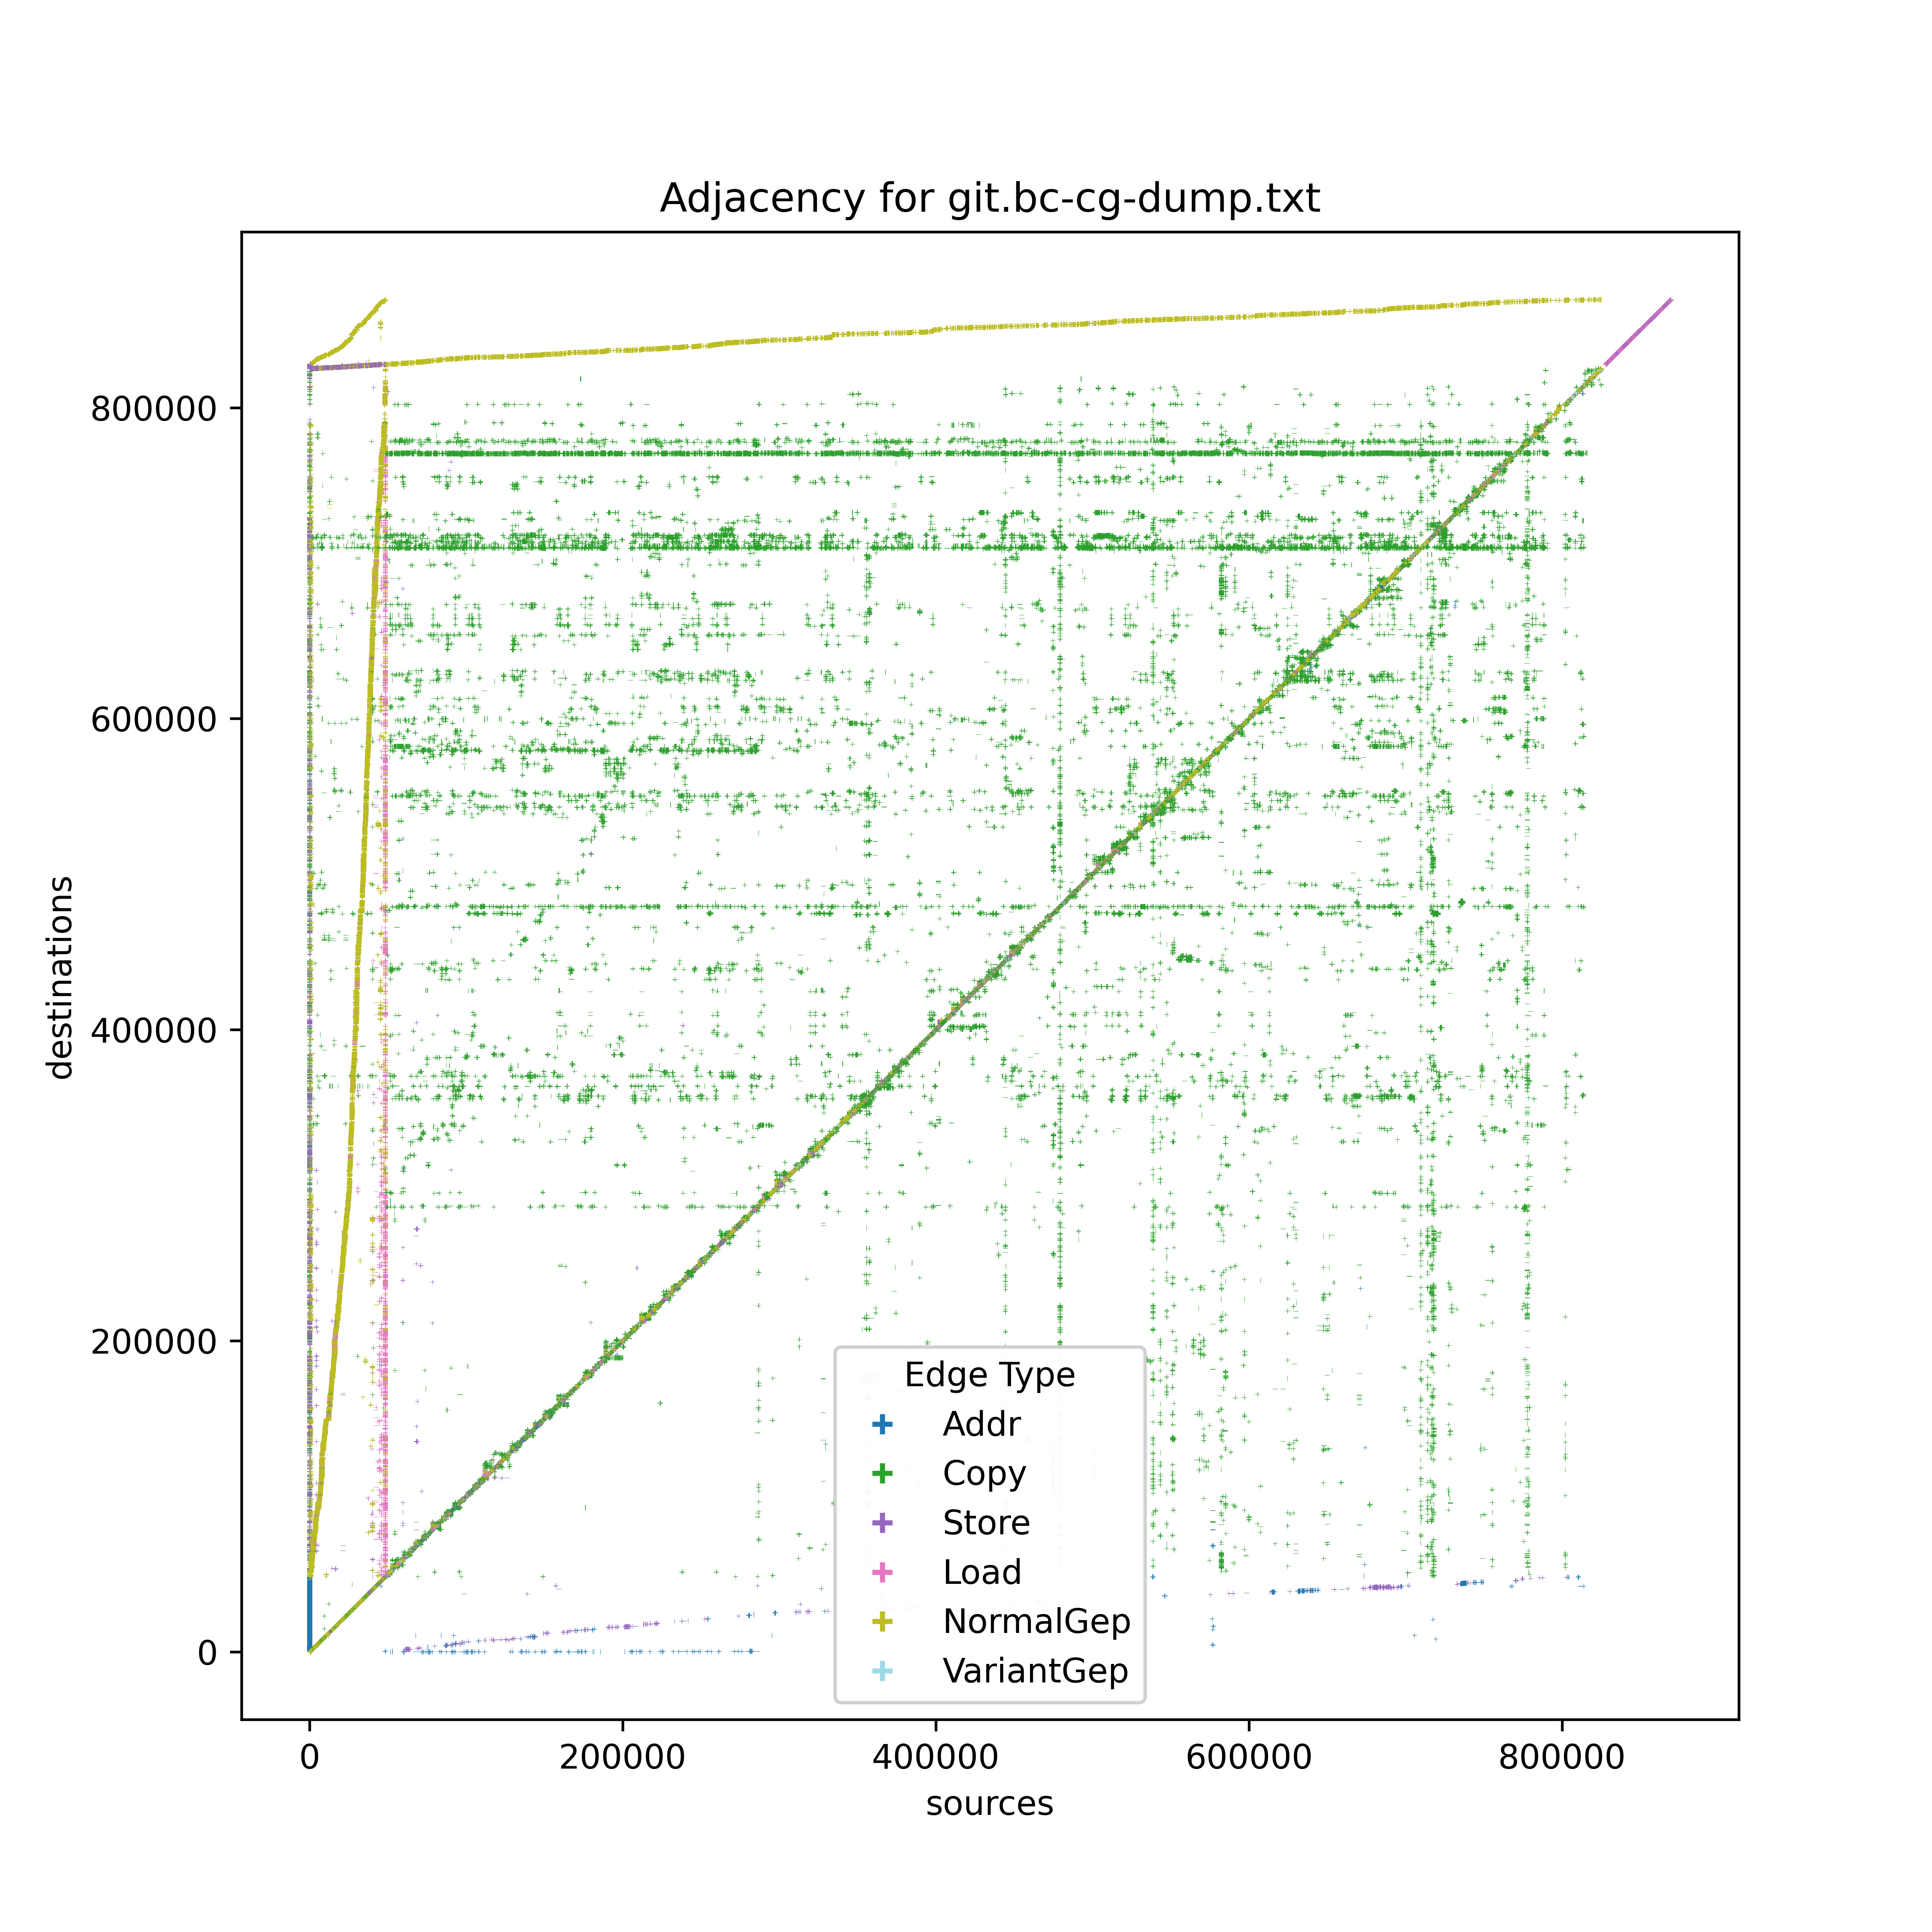
\includegraphics[width=.7\textwidth]{img/plot-git.bc-cg-dump.txt-min.png}
    \caption{Adjacency Plot for the Constraint Graph of the Git Client}
    \label{fig:git-consg}
\end{figure}

\begin{figure}[ht]
    \centering
    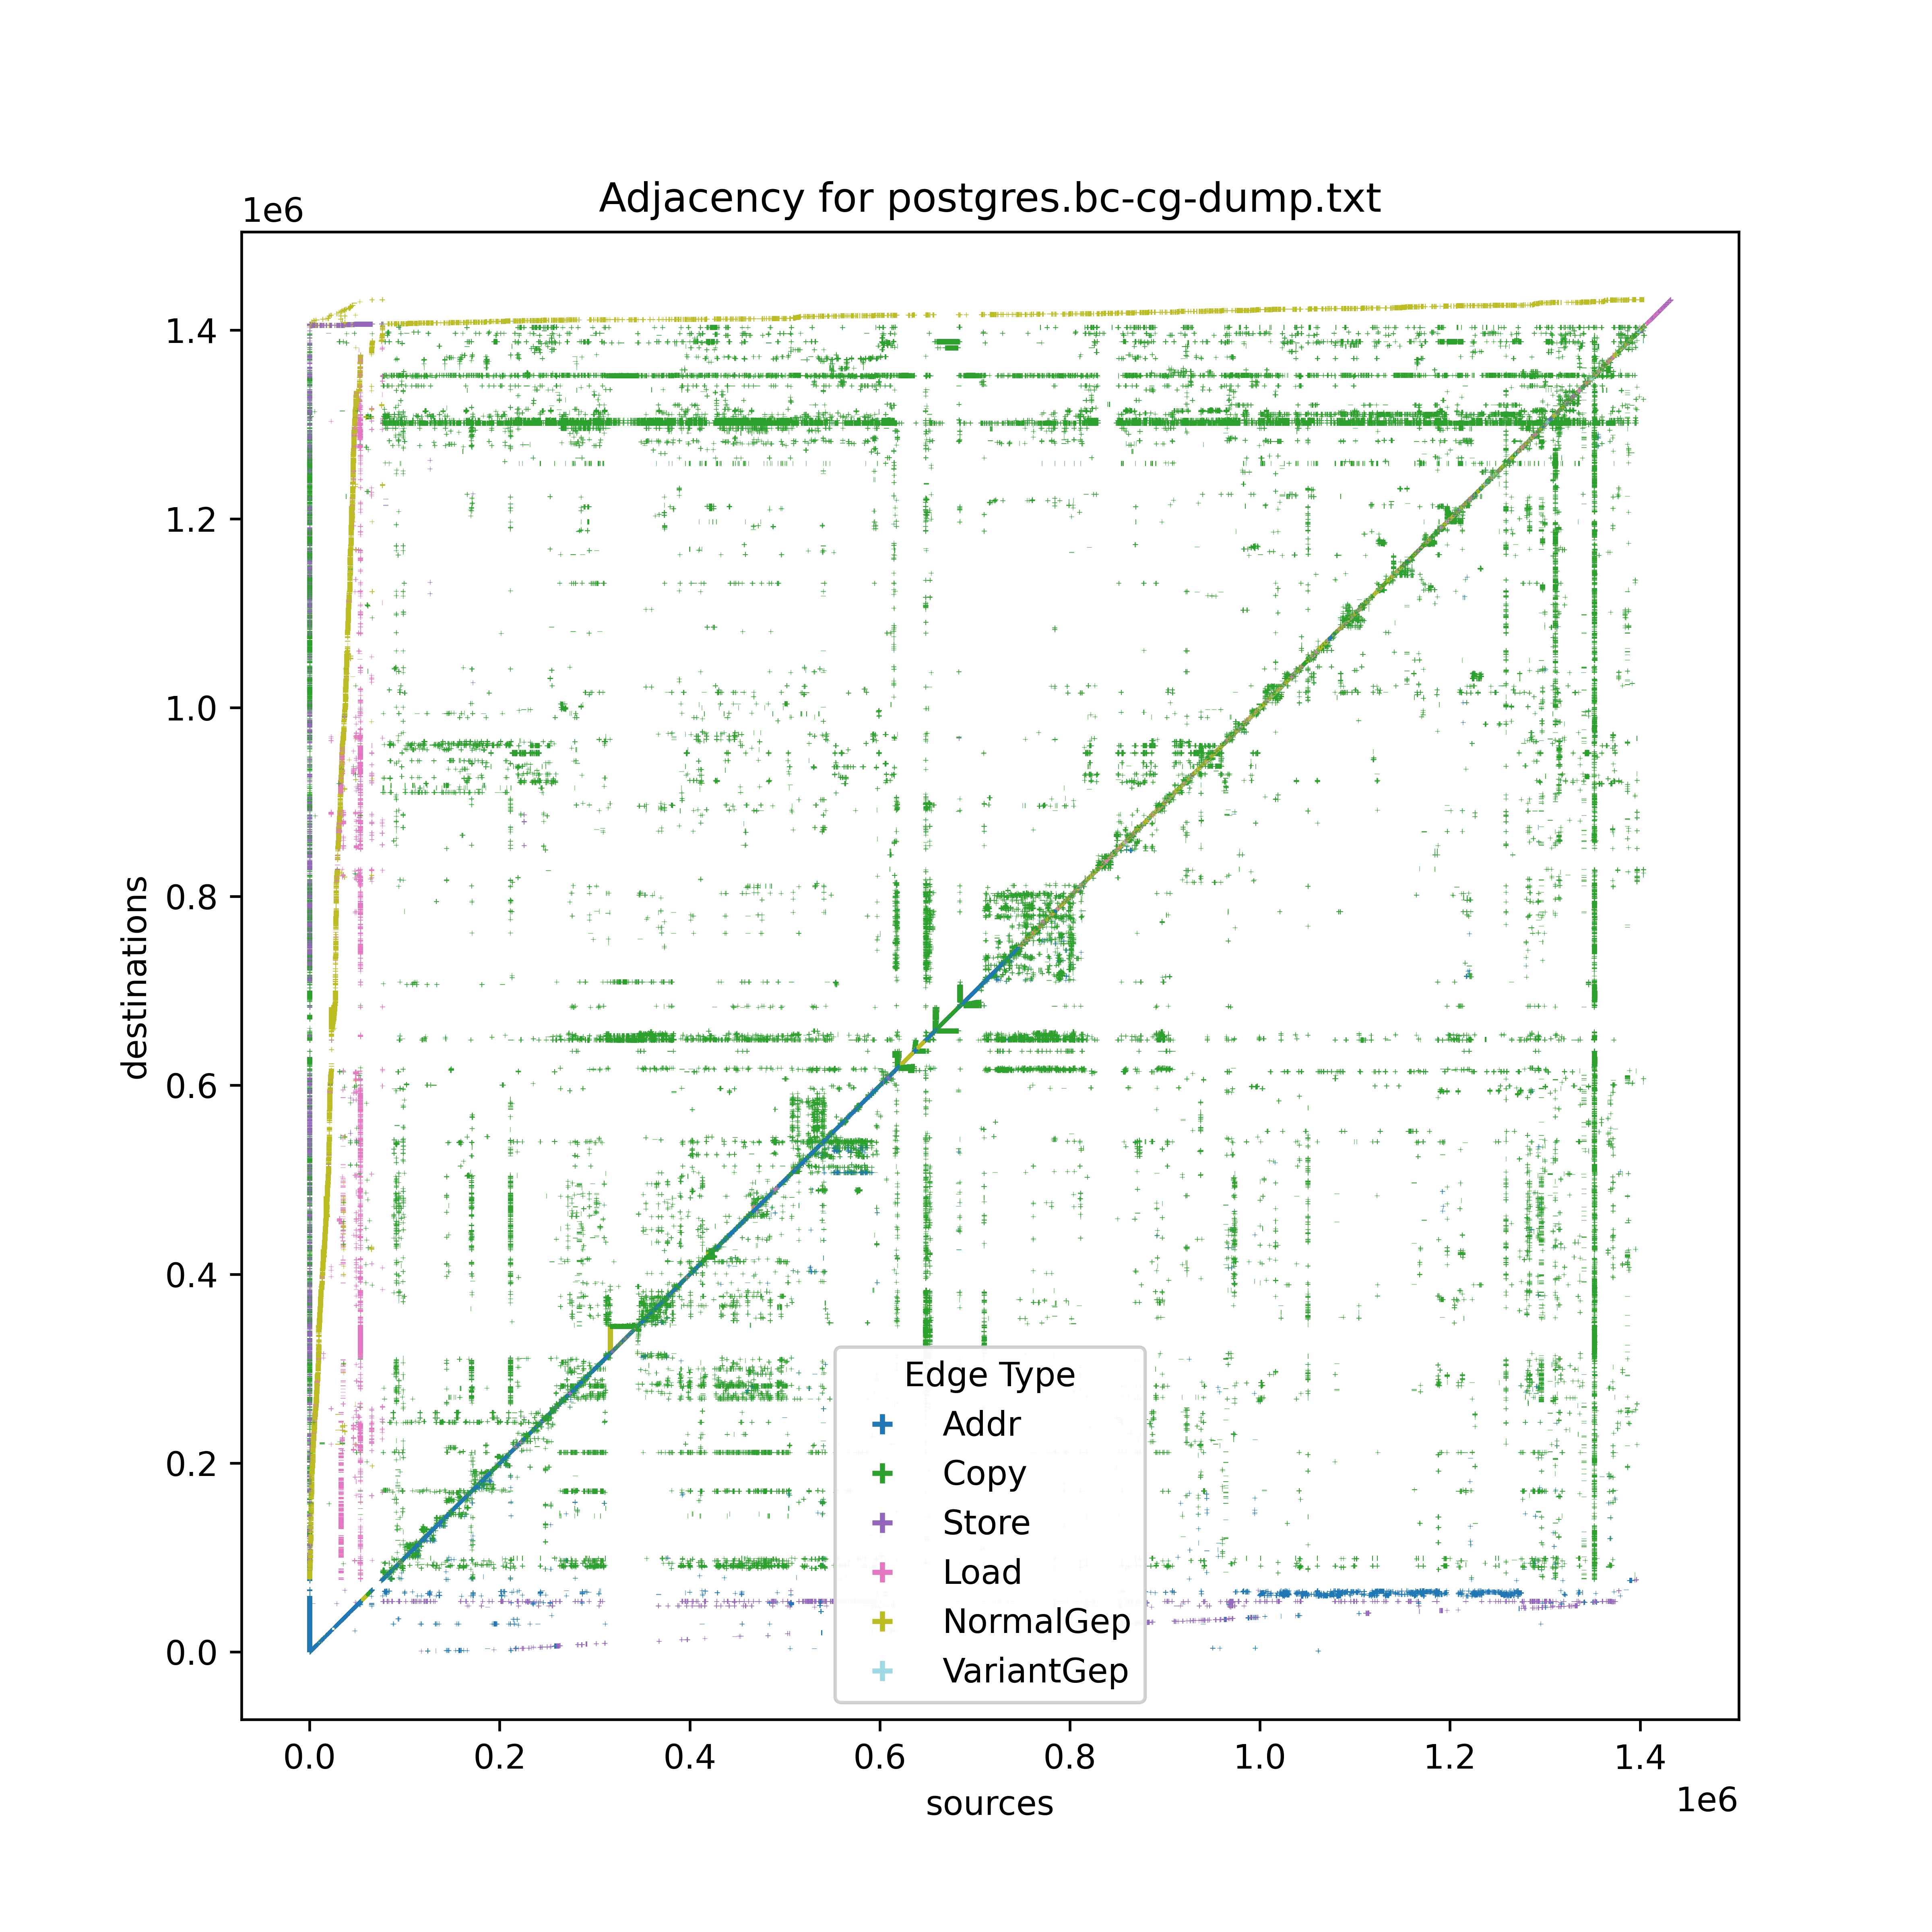
\includegraphics[width=.7\textwidth]{img/plot-postgres.bc-cg-dump.txt-min.png}
    \caption{Adjacency Plot for the Constraint Graph of Postgres}
    \label{fig:postgres-consg}
\end{figure}
